\section{Description des observations photométriques}
%

\subsection{Instrumentation}
% Brève description de l'instrumentation utilisée : télescope, spectrographe, caméra CCD
Nos mesures proviennent du télescope de Newton IRIS, situé à L'observatoire de Haute-Provance et équipé d'une caméra CCD FLI Proline 4240.

\subsection{Observations}
\subsubsection{Objets astrophysiques}
% Brève description des observations astronomiques réalisées : pour le ou les objets cibles inclure :
%  * un diagramme d'observabilité
%  * une carte de champ large en indiquant l'étoile observée sur les cartes téléchargées à https://www.iau.org/public/themes/constellations/
%  * une carte de champ resserrée produite avec Aladin ou pyastroplan et couvrant un champ de 2°x2°
%  * un bref commentaire sur l'utilité de ces graphiques
% * Un journal des observations : temps de pose, Nb ADU sous forme de description et/ou de tableau

Pour ce projet, nous avons observé l'amas ouvert d'étoiles M39 découvert en 1764 par Charles Messier, situé dans la constellation du Cygne.

\vspace{3mm}

Pour la carte de champ resserrée, il est intéressant de visualiser l'image que nous avons obtenue dans un filtre donné.
La carte resserrée présenté sur la Figure \ref{carte_M39} a été obtenue en affichant les données acquises par le CCD pour un temps d'exposition 5 secondes.

\begin{figure}[h]
    \centering
    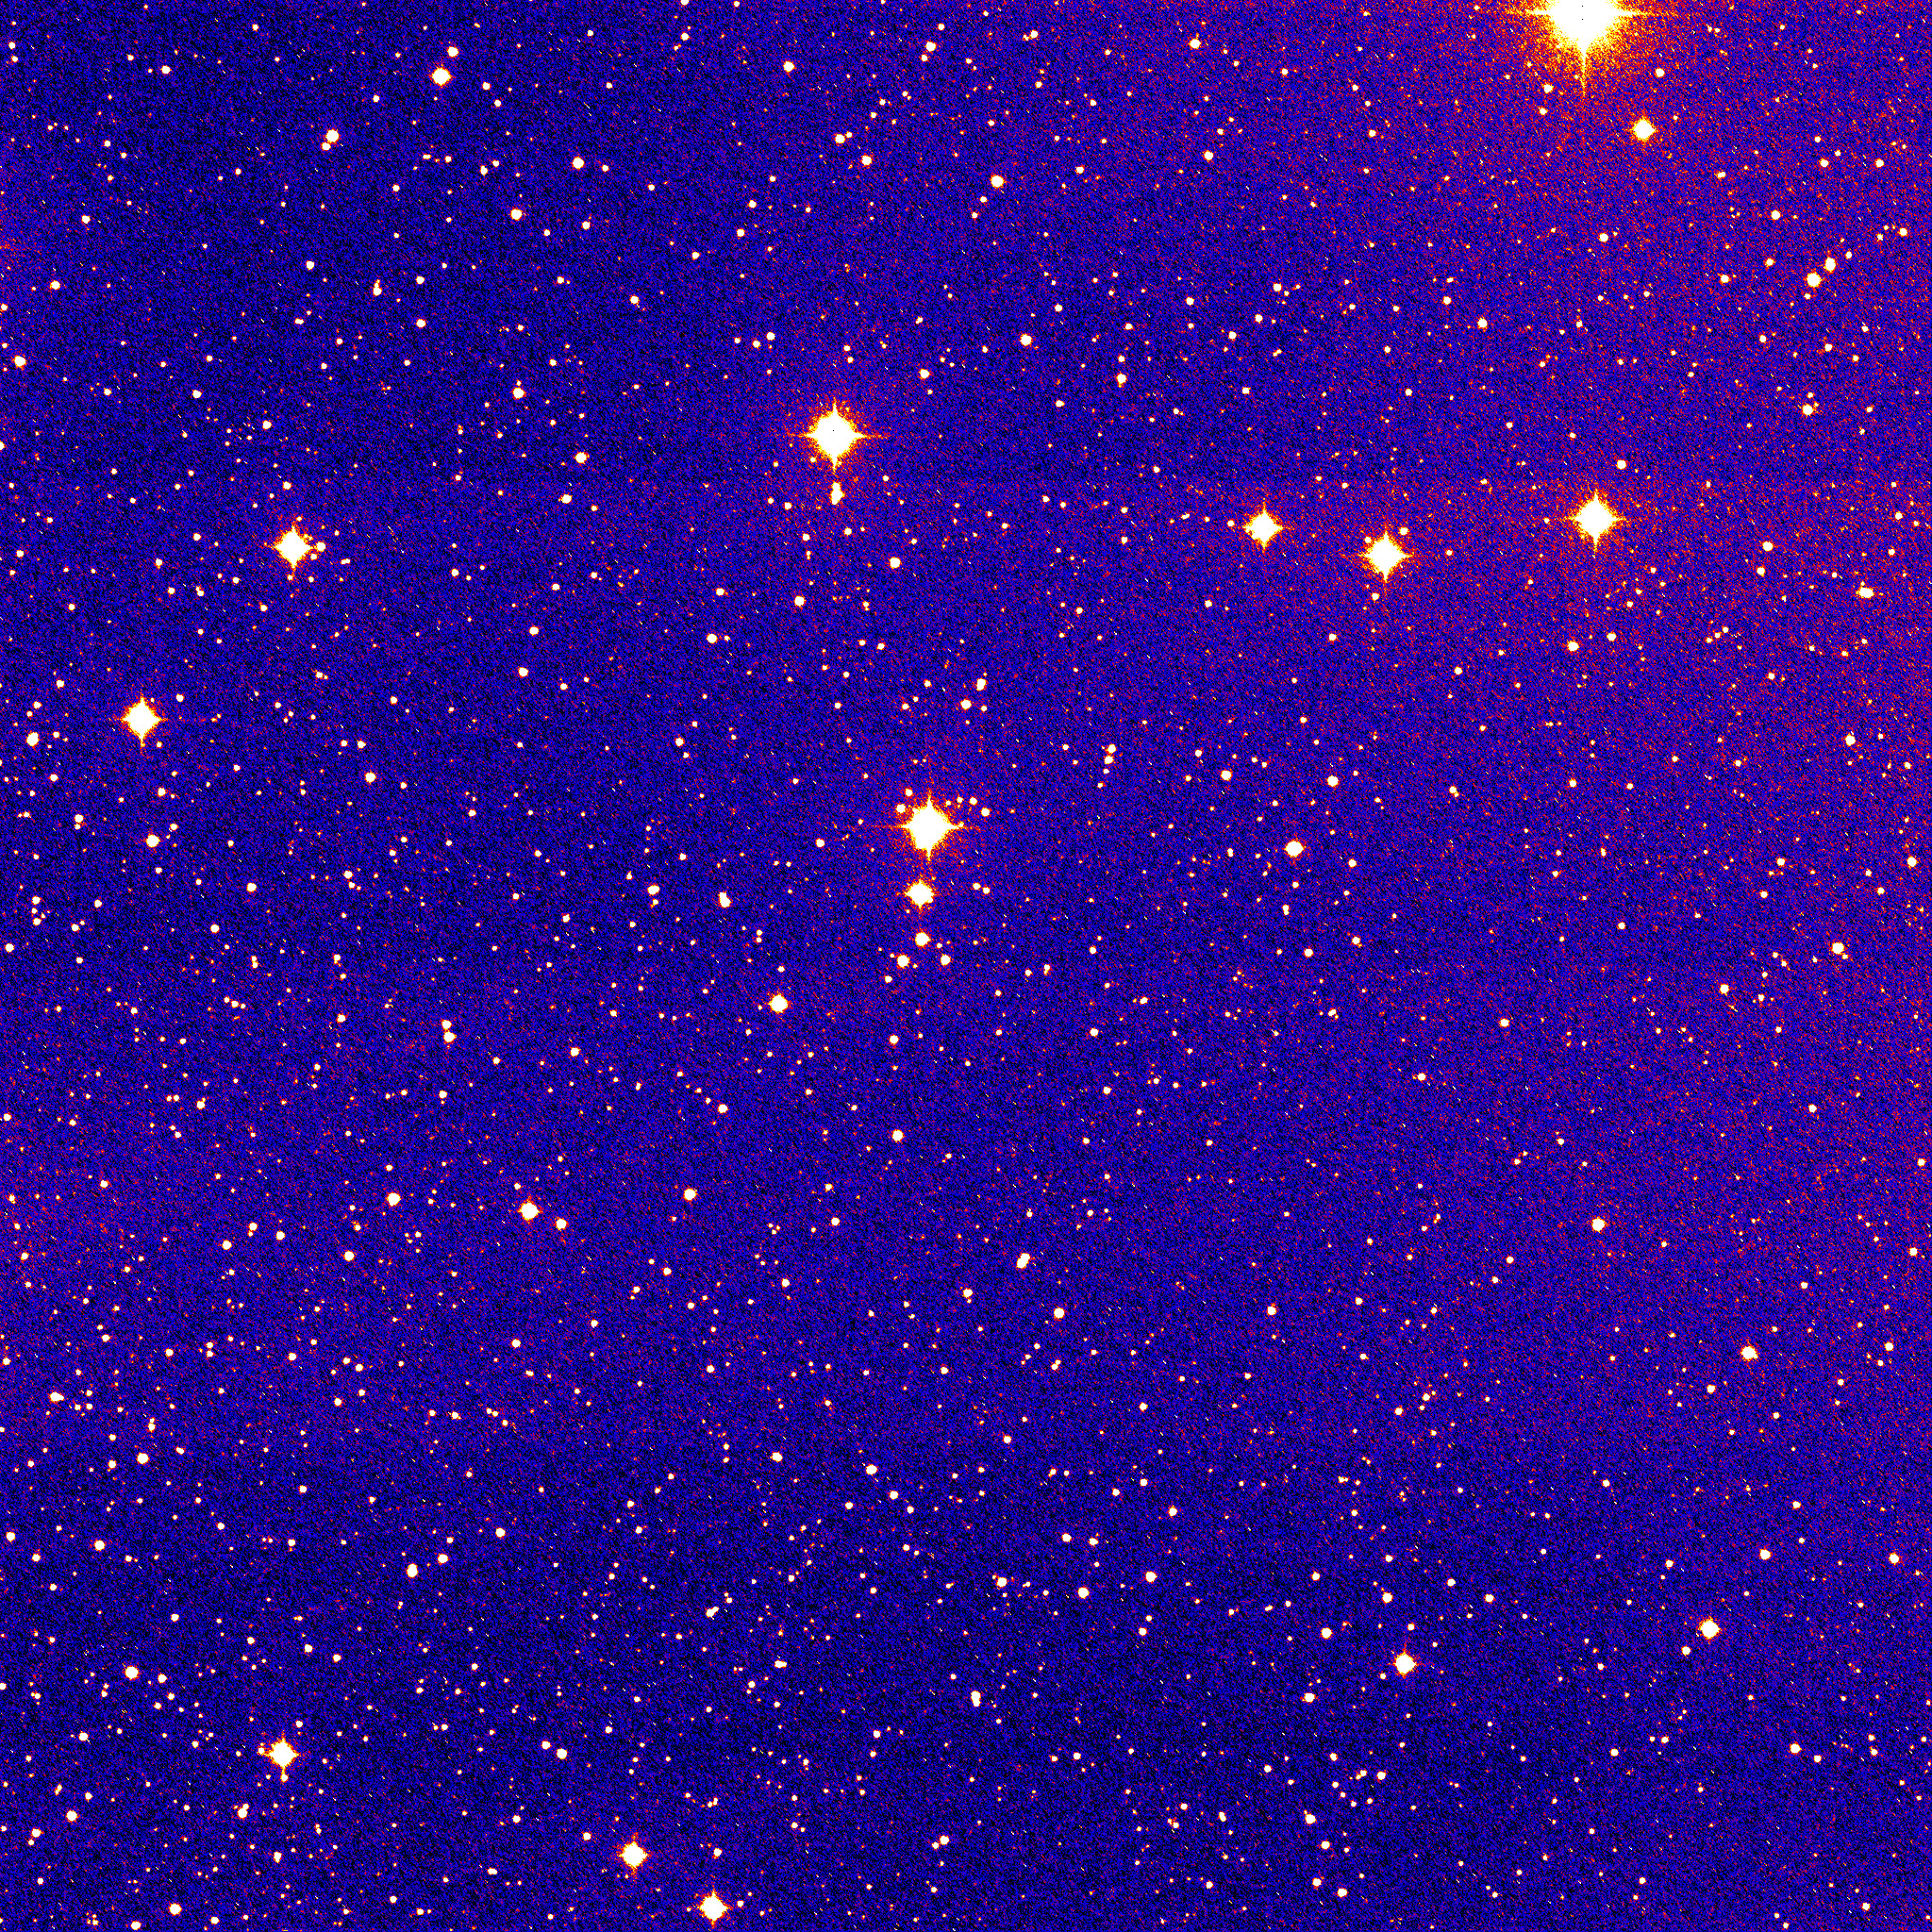
\includegraphics[width=0.5\linewidth]{fig/cover.jpg}
    \caption{Carte resserrée de M39 (filtre r)}
    \label{carte_M39}
\end{figure}


\subsubsection{Images de calibration}
% Description détaillée des différentes images acquises

Deux images ont été acquises, une image avec un filtre SDSS g , et une autre avec le filtre SDSS r.
On peut donner une valeur représentative de la longueur d'onde de filtrage de r et g avec leur valeurs centrales, données sur le [1].
On a donc :
\begin{equation}
    \lambda_r = 616.5 \ nm \ ; \ \lambda_g = 468.6 \ nm
\end{equation}

Le temps de pose de chaque image est toujours de 5 secondes. Pour le lecteur intéressé, toutes les données supplémentaires sur les images se trouvent dans le Notebook Jupyter et dans le Header de l'image.

\subsubsection{Caractérisation de la caméra CCD}
% Caracterisation de la caméra CCD : gain (e-/ADU), bruit de lecture (e-), courant d'obscurité % (e-/s/pix)
% Expliquer comment ces grandeurs sont déterminées et comparer aux données constructeur
% Expliquer brièvement à quoi correspondent ces grandeurs

Une caméra CCD (Charged Coupled Device) est un récepteur multicanal, constitué d'un "pavage" d'électrodes (ou pixels récepteurs) dans une certaine plage de longueur d'onde. 

La caractérisation de notre CCD est importante car elle permet d'obtenir toutes les données importantes sur celui-ci. 
Toutes ces données se trouvent dans la fiche fabricant et certaines données calculées se trouvent dans le Header. Notre CCD, est donc caractérisé par les données sur la Table \ref{CCD}.
% gain, bruit de lecture, courant d'obscurité, position du télescope, 
\begin{table}
    \centering
    \begin{tabular}{|c|c|}
        \hline
        Surface de l'image (diagonal) & $27.6 \times 27.6 \ mm$ \\
        \hline
        Nombre de pixels & $2048 \times 2048$ \\
        \hline
        Capacité maximale & $10^5$ e- \\
        \hline
        Taille d'un pixel & $13.5 \times 13.5 \ \mu m$ \\
        \hline
        Courant d'obscurité & $0.2$ e-/s à $-30^\circ C$ \\
        \hline
        Refroidissement maximal & $60^\circ C$ \\
        \hline
        Bruit de lecture & $14.32$ e- \\
        \hline
        Gain théorique & $1.35$ e-/ADU \\
        \hline
        Gain & $1.339$ e-/ADU \\
        \hline
    \end{tabular}
    \caption{Données de la caméra  [2]}
    \label{CCD}
\end{table}

La caméra CCD est composée de plusieurs pixels chacun mesurant des photons, puis par effet photo-électrique, ils sont convertis en électrons. Ce sont les électrons qui nous permettent d'exploiter le signal.

\vspace{3mm}

Or, lors de l'effet photo-électrique, des photons nuisibles peuvent être produits par l'agitation thermique et contribuer au bruit de lecture.
Pour empêcher au maximum cet effet, on refroidit la caméra. Le bruit de lecture donné ici est donc le bruit de lecture à $-25^\circ C$, déterminé grâce à un flux de calibration parfaitement connu.
Le bruit de lecture vient aussi du courant d'obscurité, faible ici dans notre cas (nos images ont des temps de pose de l'ordre de 5s).
%explication du dark current

\vspace{3mm}

La résolution de notre image est simplement la taille d'un Plus un pixel est petit et plus l'image sera précise. Ici, nous sommes à l'ordre du micromètre.
Après un temps de pose, le CCD accumule des électrons dans chaque pixel (qui est en fait un puits quantique grâce à la tension appliquée).
Mais, si le nombre d’électrons est trop grand, chaque pixel peut "fuiter" sur d'autres pixels. 
En d'autres termes, s'il y a trop d’électrons dans un puits quantique, certains électrons vont réussir à s'échapper pour passer au suivant.
La caractéristique de la capacité maximale, nous renseigne le nombre d’électrons où nous pouvons commencer à percevoir des fuites, et est facilement déterminer par des calculs ou mesures.

\vspace{3mm}

Le gain du CCD nous permet de mesurer l'effet de l'amplificateur sur le signal mesuré en électrons. Il convertit donc ce qu'on reçoit (les électrons) en ADU. 
Lors de la prise d'une image, le CCD calcul le gain réel, nous prendrons donc cette valeur dans la suite de nos mesures